\chapter{Proposed Translator}
\label{ch:proposed-translator}

This chapter focuses on proposing a solution to ODMTP.
First formalizing the solution. And then modelling it
with elements of software engineering such as use cases
and requirements.

\section{Translator Formalization}
As a solution to the previous chapter, this section focuses on
proposing a application $f : S' \rightarrow M$ such that
applied on a schema, results in a domain model based on
plain objects.

Lets define $f(S') = \begin{bmatrix}f'(s_1')\\ f'(s_2')\\ \vdots\\ f'(s_n')\end{bmatrix}$ and
$f'(s_i') = \begin{bmatrix}f''(e_1')\\ f''(e_2')\\ \vdots\\ f''(e_n')\end{bmatrix}$. Then $f''(e_i')$
is the application that maps a triple expression $e'$ from $N \times T_{g} \times \{(1,1),(0,\infty)\}$
to $N \times T_g$. To find such a function we will use the knowledge that we already have.
We know that $p$ has a direct mapping as it belongs to $N$, $T_g$ maps to $T_g$ if
the cardinality value is $(1,1)$ or $(1, \infty)$. And the cardinality is aggregated to the type
so its not needed to map it. Then we define the application $f''(e')$ as $f:(p,t,c) \in N \times T_g \times \{(1,1), (0,\infty)\} \rightarrow (n,t)\in N \times T_g$
and therefore,

\begin{equation}
f''(e_i')
\begin{cases}
    (p,Proy_{t_g}lst) & if \; c=(1,1) \\
    (p,List[Proy_{t_g}lst]) & if \; c=(0,\infty)
\end{cases}.
\end{equation}

This application's function is to transform a triple expression
into an annotated type property. Where the $Proy_{tg}lst$ represents
the projection of the generic type from the abstraction of languages
of representation of plain objects on to the language specific type.
\cref{fig:lst-diagram} illustrates how the same input can lead to
multiple types due to the specific translators, that perform the 
$Proy_{tg}lst$ operation.

\begin{figure}
    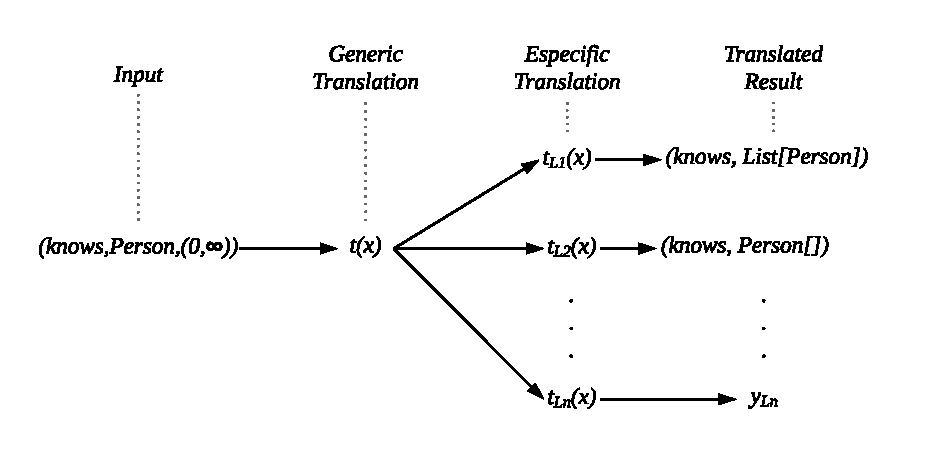
\includegraphics[scale=0.8]{images/lsc-diagram.pdf}
    \centering
	\caption[Different target types generated by specific translators]{Different target types generated by specific translators.}
    \label{fig:lst-diagram}
\end{figure}

\section{Translator modelling}
This section focuses on modelling through use cases and requirements
a system that implements the transformation function described in the
previous section.

The following use case diagram models the different scenarios and
behaviour that the translation the system should be able to support.
\begin{figure}[h!]
    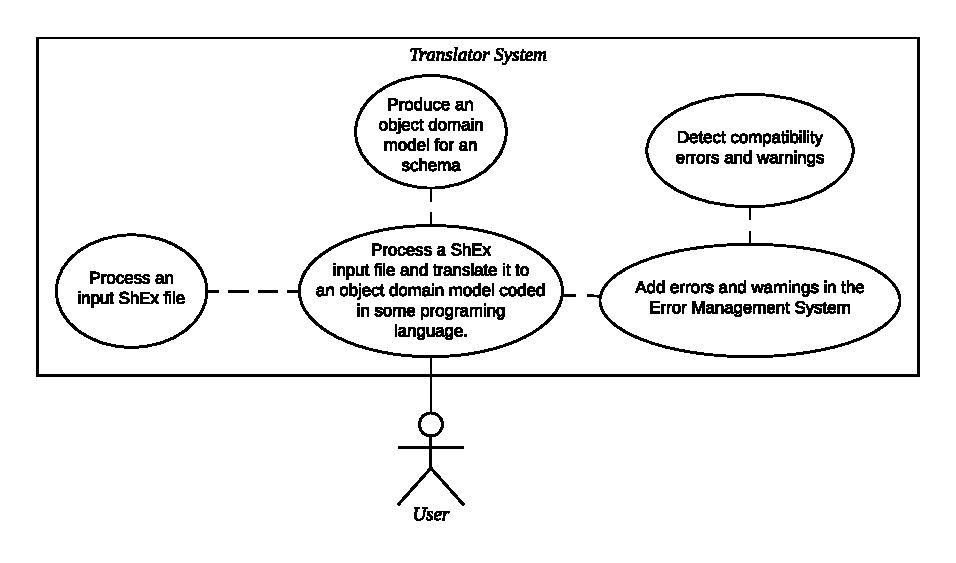
\includegraphics[scale=0.8]{images/trans-use-case.pdf}
    \centering
    \caption[Translator use cases]{Translator use cases.}
    \label{fig:trans-use-case}
\end{figure}

From the previous use cases we can extract some functional and non functional requirements.

\begin{figure}[h!]
    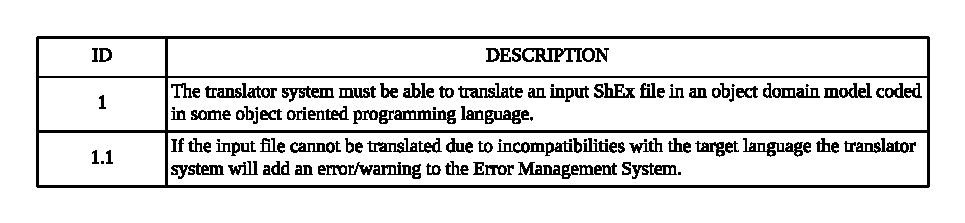
\includegraphics[width=\textwidth]{images/trans-reqf.pdf}
    \centering
    \caption[Translator functional requirements]{Translator functional requirements.}
    \label{fig:trans-reqf}
\end{figure}

\begin{figure}[h!]
    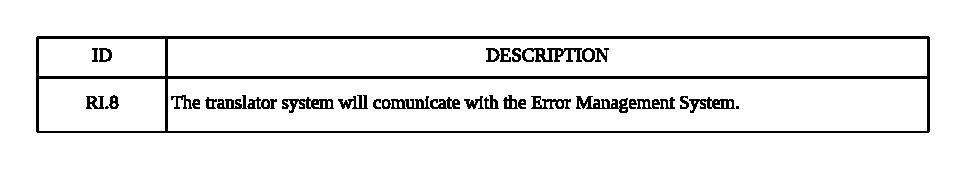
\includegraphics[width=\textwidth]{images/trans-reqnf.pdf}
    \centering
    \caption[Translator non functional requirements]{Translator non functional requirements.}
    \label{fig:trans-reqnf}
\end{figure}

Thus, for the previous use cases and requirements the implementation abstract diagram will be.

\begin{figure}[h!]
    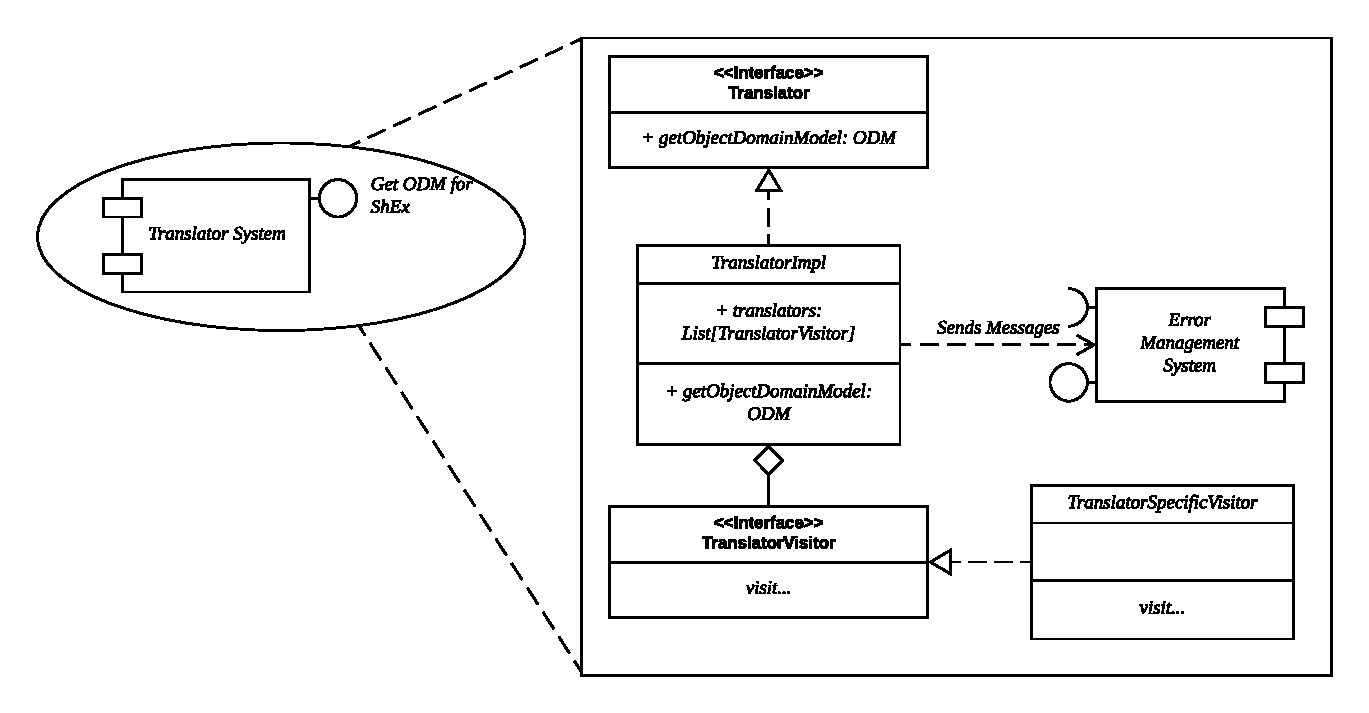
\includegraphics[width=\textwidth]{images/trans-diagram.pdf}
    \centering
    \caption[Translator component and class diagrams]{Translator component and class diagrams.}
    \label{fig:trans-diag}
\end{figure}